\chapter{Server}
\label{ch:server}

\todo{what are servers?}

\section{History of Servers}

\todo{what were the first approaches to servers? how are they used?}

\section{Tasks}
The tasks of the server are to manage incoming connection and their requests. It should always be prepared to send sensor data to a client if it is requested.
\section{Hardware}
\subsection{Raspberry Pi 3 Model B}
The Raspberry Pi is a small single-board computer originally created to teach children how to program \cite{RasPi}. It was developed by the Raspberry Pi Foundation. There are numerous options for expanding the capabilities of the Raspberry Pi. One being the use of General-purpose input/output (GPIO) pins. These can be used by so-called HAT's (Hardware Attached on Top) or Shields (this term evolved from Arduino-land). These add-on boards are mounted to the Raspberry Pi by connecting the GPIO pins to the board and screwing them together. They mostly provide additional hardware that can be used to achieve the desired goal. Further advantages are its relatively small footprint and its low cost. Also, a wide variety of Linux distributions have been adapted to the hardware. Having these advantages was the decisive factor for choosing the Raspberry Pi 3 Model B.\\
The specifications of the Raspberry Pi 3 Model B are:

\begin{itemize}
	\item \textbf{SoC} Broadcom BCM2837
	\item \textbf{CPU} 4x ARM Cortex-A53, 1.2GHz
	\item \textbf{GPU} Broadcom VideoCore IV
	\item \textbf{RAM} 1GB LPDDR2 (900 MHz)
	\item \textbf{Networking} 10/100 Ethernet, 2.4GHz 802.11n wireless
	\item \textbf{Bluetooth} Bluetooth 4.1 Classic, Bluetooth LE
	\item \textbf{Storage} microSD
	\item \textbf{GPIO} 40-pin header, populated
	\item \textbf{Ports} HDMI, 3.5mm analogue audio-video jack, 4x USB 2.0, Ethernet, Camera Serial Interface (CSI), Display Serial Interface (DSI)
\end{itemize}

\subsection{Raspberry Pi SenseHAT}

During the first implementation phase a Raspberry Pi SenseHAT add-on board was used the get real sensor data \cite{SenseHAT}. This HAT was made especially for the Astro Pi mission, where student could create and code projects, which were then run on the International Space Station by astronaut Tim Peake \cite{AstroPiMission}. This board was chosen because it offers a wide variety of sensors and therefore offers many possibilities in terms of testing GRAMOC.

The Raspberry Pi Sense HAT includes following sensors and inputs/outputs:

\begin{itemize}
	\item ST LSM9DS1 Inertial measurement sensor
		\begin{itemize}
			\item 3D accelerometer
			\item 3D gyroscope
			\item 3D magnetometer
		\end{itemize}
	\item ST LPS25H barometric pressure and temperature sensor
	\item ST HTS221 relative humidity and temperature sensor
	\item Alps SKRHABE010 5-button mini-joystick
	\item 8x8 RGB LED matrix
\end{itemize}
\bigskip
The RGB LED matrix and the joystick are both driven by a Atmel ATTINY88 microcontroller-unit.\\
Because this project focuses on data from magnetic field sensors, the focus was put onto the 3D magnetometer of the SenseHAT. This sensor has a magnetic measurement range of $\pm$ 4/8/12/16 gauss \cite{InertialSensorsManual}.

\subsection{Magnetic field sensors}

\todo{what are magnetic field sensors, what do the measure, how do they measure}

\section{Implementation}

\todo{more precise}
The server program of GRAMOC is written in Python. This allows for great compatibility.

\subsection{Programming Language}

\todo{explain why Python was chosen, differences between 2 and 3, why 3?}
Python is a simple yet powerful, modern programming language and supports both procedure-oriented as well as object-oriented programming. It was developed by Guido van Rossum at Centrum Wiskunde \& Informatica (CWI) in the Netherlands in 1989 and first released in 1991 \cite{HistoryOfPython}. It was meant to be a successor to the ABC programming language. Since Python is a high-level language, it automatically manages the memory used by the program.

\section{Program Flow}

As depicted in figure \ref{fig:server-program-flow}, the server starts accepting new connections right after is has started. It then performs the handshake that is required by GSDEP (further explained in \ref{sec:networking_data-flow}). If this handshake is performed without errors, the server starts listening for data from this now connected client on a separate thread. While this thread is running it receives one message and checks if it is a command (see \ref{sec:networking_command}). If it is, the message is interpreted and the appropriate function is executed. This thread is kept alive until the client disconnects or the server is shutdown by the user.

\begin{figure}[H]
	\centering
	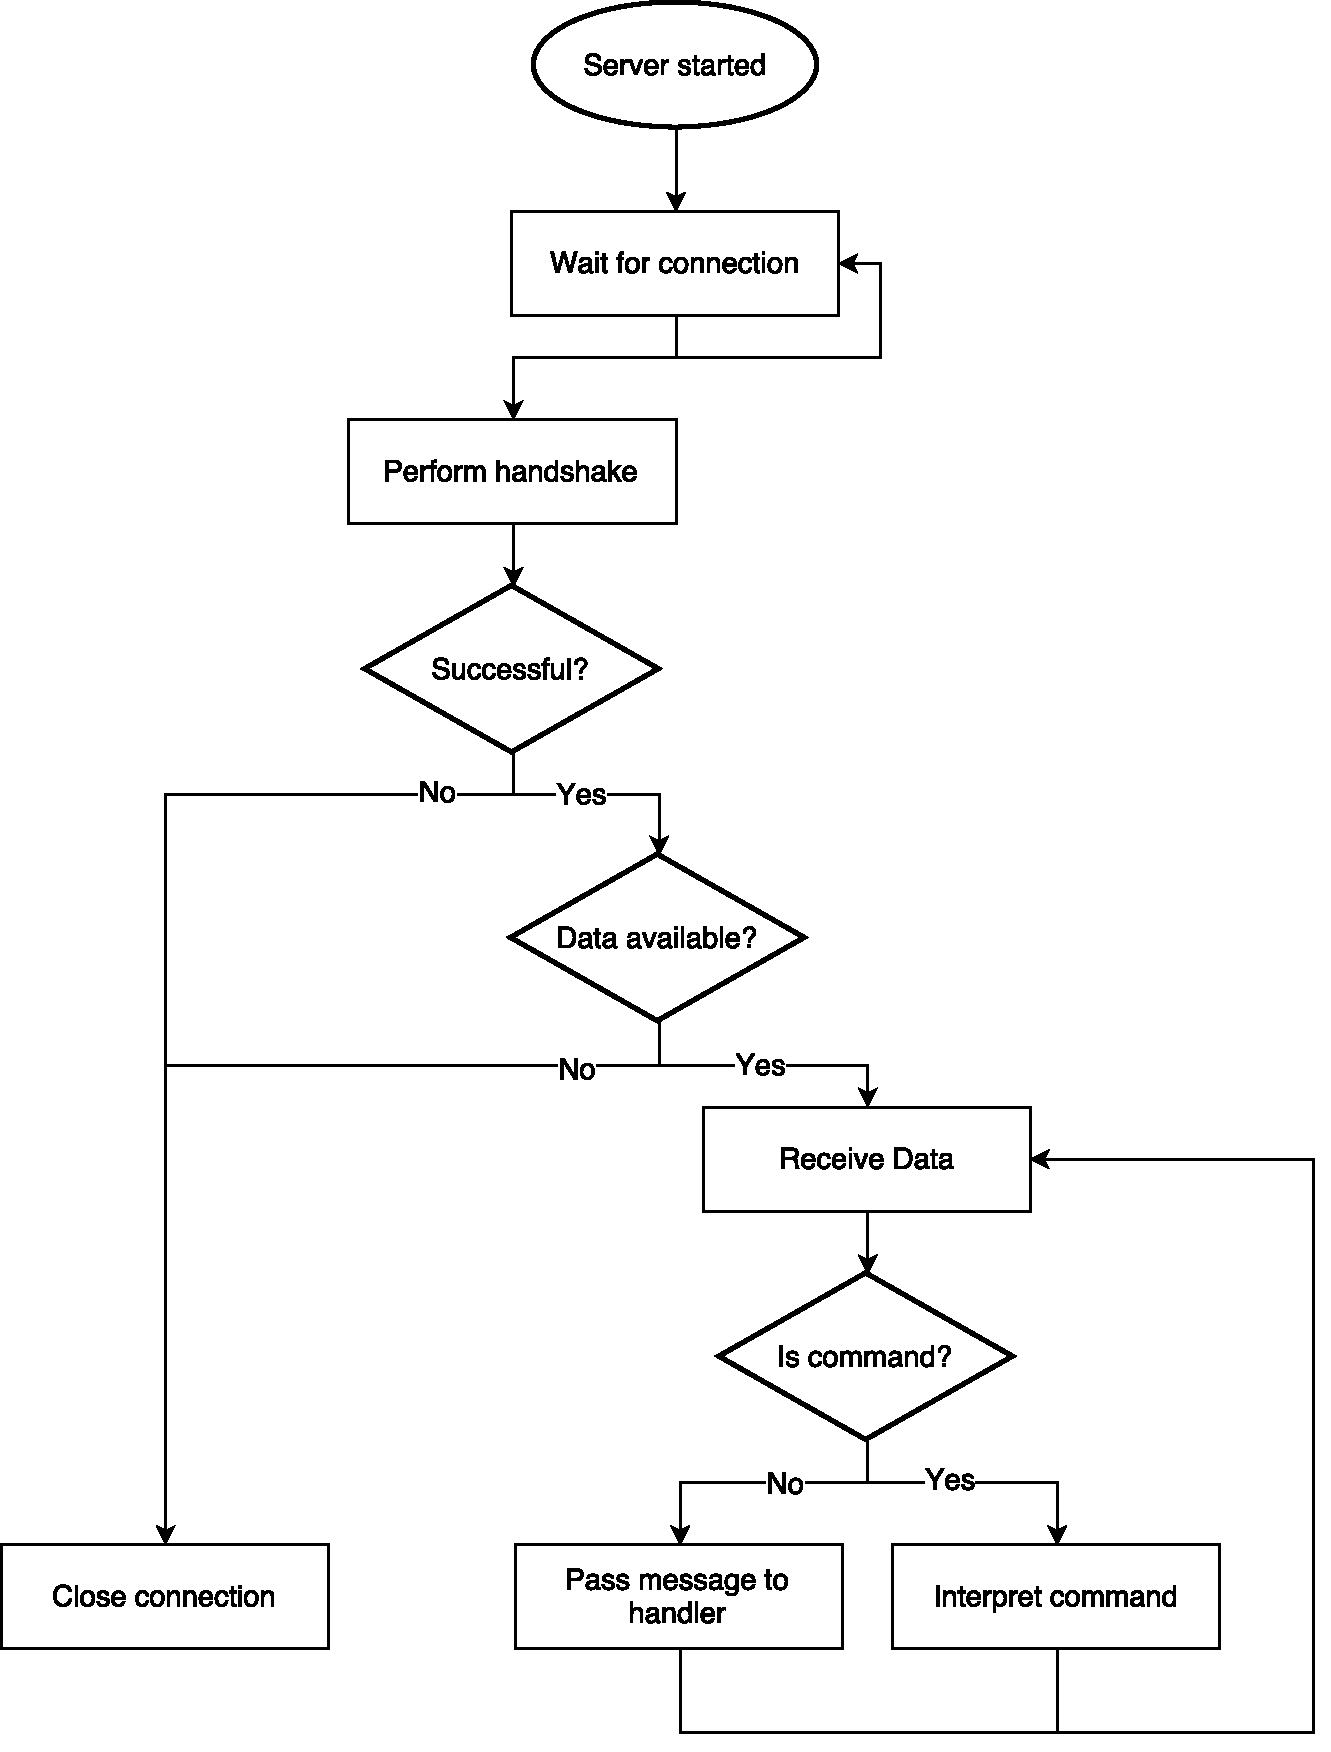
\includegraphics[width=8cm,keepaspectratio]{server-task}
	\caption{Flowchart of server program showing the procedure}
	\label{fig:server-program-flow}
\end{figure}
